\section{Asure Network}

The Asure network consists of the node clients in which the Asure blockchain is operated and synchronized among the individual nodes with the help of the consensus. To achieve the number of required transactions, the load must be distributed over several blockchains. One or many blockchains can be specific for a single social security system.  In order to benefit from the blockchain ecosystem, and the great added value for scalability arises only when the assets can be transferred among the several blockchains. Also, specialized side-chains can benefit from the security of the root-chain and thus the assets are better protected. \cite{omisego}

\subsection{Requirements}
The core social security and blockchain requirements in a scalable scenario are as follows:

\subsubsection*{Transaction Throughput}
The Asure network must be able to scale transaction throughput through side-chains to such an extent that countries and residents can do their financial transactions within the off-chain.

\subsubsection*{Privacy}
In order to protect the privacy of the users, no private data may be stored on the blockchain. If possible, transactions should not be assigned to a user. Personal data is encrypted and stored outside of the blockchain. By using the Zero-Knowledge-Proof method, the storage of personal data can be completely avoided. 

In order for a blockchain-based social security to be established, it must comply with the data protection and privacy guidelines of national and international regulations such as the General Data Protection Regulation (GDPR) in the European Union. \cite{gdpr}

\subsubsection*{Transparency}
Transparency within the Asure network is an important factor to protect social security systems against corruption and manipulation. While respecting the privacy of the users, it is important to ensure transparency of the system, in general, to enable for example real-time statistics of the overall money-flow.

\subsubsection*{Business rules for the system}
Social security has many influencing factors and rules, these must be fulfilled, adapted and executed, therefore it is our requirement to be able to execute custom business rules in the side chain with EVM or EWASM.

\subsubsection*{Security}
A system that organizes and stores the financial transactions of social security systems must satisfy multiple security requirements. It must be ensured that data cannot be manipulated or stolen and the system is resistant to attacks, breakdown, and other failures.

\subsection{Further technologies}
Poon and Buterin presented the Plasma framework in 2017 to solve the scaling problem by arranging multiple independent blockchains into a tree hierarchy. Consecutive Plasma proposals have described off-chain venues for simple transfers of fungible and non-fungible tokens. These proposals include Plasma MVP, Plasma Cash, and Plasma Debit. The Plasma framework is under active research and depending on the application and requirements the plasma implementation varies.\cite{plasma} Loom and OmiseGO are one of the first who implements plasma and continues their research in this field. 

Plasma was introduced very recently and is among the more promising proposed solutions to scalable computation on the blockchain. The Plasma whitepaper is very broad and doesn’t have all the technical information necessary for immediate implementation. Plasma can provide scalability for Ethereum applications. It is an application-specific side-chain protocol.

Polkadot, on the other hand, was presented by Gavin Wood in 2017. The aim of the concept is to create a heterogeneous multi-chain solution that enables the connection of individually adapted side-chains with public blockchains. Polkadot allows different blockchains to exchange messages in a secure and trustworthy way.

The Raiden Network is an off-chain scaling solution with payment and state channel technology, enabling near-instant, low-fee and scalable payments. It’s complementary to the Ethereum blockchain and works with any ERC20 compatible token.

\subsection{Plasma}
The Asure network will use the Plasma framework to create a scalable blockchain network for social security systems requirements. 

To raise the limits of Layer 1 even further in order to effectively operate the social security system, Layer 2 scaling is considered to be the most efficient solution. It makes it easier to implement security in the system as it relies on Layer 1. The solution will be designed as a combination of Asure root-chain and corresponding side-chains to match social security systems needs.

Asure side-chains can be connected to smart contracts of Ethereum or any other blockchain technologies which are working with Plasma design patterns.


\begin{figure}[H]
    \centering
    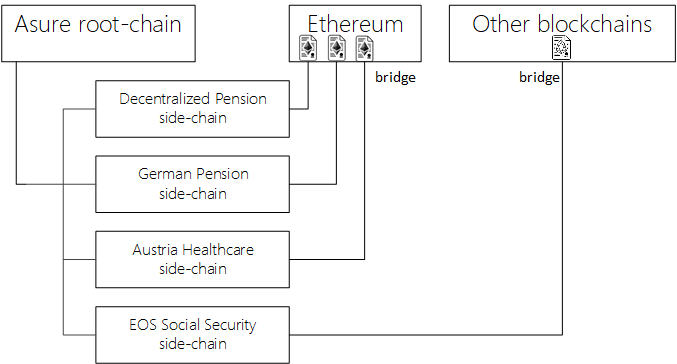
\includegraphics[width=4.0in]{img/chains.png}
    \caption{Asure side-chains}
    \label{fig:asure_side_chains}
\end{figure}
